\documentclass[11pt]{article}
\usepackage{mathptmx}
\usepackage[margin=1in]{geometry}
\usepackage{graphicx,amsmath,amssymb,url}
\setlength{\parskip}{4pt}\setlength{\parindent}{0pt}
\title{Non-conserved microRNA targeting at scale: a duplex-aware CNN beats context-augmented baselines, rediscovers the ciRS-7 sponge, and survives CLIP falsification}
\author{MEGA27 Project 18}
\date{September 2026}
\begin{document}\maketitle
\begin{abstract}
Canonical miRNA target prediction restricts itself to evolutionarily conserved sites, leaving the non-conserved majority of the targetome unranked. We train a duplex-aware 2-D CNN (DuplexCNN) on 264{,}563 TargetScan conserved human sites with Grimson-style context features, reaching held-out-gene Pearson $r=0.811$ vs $0.779$ for a ridge model on identical features and $0.664$ for sequence-only ridge. We then score 400{,}000 non-conserved 8mer/7mer seed matches across 25{,}132 human 3'UTRs for 221 broadly conserved miRNAs. The top-scoring pair, hsa-miR-7-5p$\to$CDR1as, is the ciRS-7 sponge interaction --- a positive control rediscovered blind. Falsification against independent AGO-CLIP data (ENCORI, 23 miRNAs, 83{,}624 pairs) shows the CNN adds a small but statistically real signal beyond seed counts, UTR length and miRNA identity ($\Delta$AUROC $=+0.0075$, 95\% CI $[0.0057,0.0093]$, permutation $p=0.048$). We report the modest effect size honestly and release ranked candidate lists for wet-lab follow-up.
\end{abstract}
\tableofcontents\newpage
\section{Introduction}
Most mammalian miRNA targeting is quantified through context++ scores on conserved sites. Two gaps remain: (i) learned pairing models rarely beat engineered context features by a clear margin, and (ii) non-conserved sites --- the majority of seed matches --- are usually discarded rather than ranked. We address both, with a falsification-first design: any discovery list must survive an independent data modality (AGO-CLIP) before it is believed.
\section{Data}
TargetScan vert\_80: 264{,}563 human conserved sites with context++ labels; 25{,}132 human 3'UTR sequences; miR family table (221 broadly conserved human miRNAs, Family Conservation $=2$). ENCORI/starBase miRNATarget API (hg38, clipExpNum$\ge1$): per-miRNA CLIP-supported gene sets for 23 panel miRNAs.
\section{Methods}
\subsection{DuplexCNN architecture}
A pairing map $P\in\{0,1\}^{4\times 4\times W}$ encodes UTR window against miRNA nucleotides; site-type embedding and normalized context features $F$ (3' pairing, local AU, position, SA per Grimson et al.) join at the head:
\begin{equation}
\hat y = w^{\top}\big[\phi_{\mathrm{conv}}(P)\,\Vert\,e_{\mathrm{site}}\,\Vert\,F\big]+b,
\qquad \mathcal L=\frac1N\sum (y_i-\hat y_i)^2 .
\end{equation}
Context features are standardized on the training split only; genes (not sites) define the 80/20 split, preventing transcript leakage.
\subsection{Non-conserved scan}
For each broadly conserved miRNA we enumerate 8mer and 7mer-A1 seed matches with zero overlap to any TargetScan conserved interval, subsample to 400k, and score with the trained model.
\subsection{CLIP falsification design}
Unit of analysis: (miRNA, gene). Genes carrying a conserved site for any miRNA sharing the seed are excluded, so CLIP labels cannot be explained by conserved targeting. Features: $\min$ and $\sum$ CNN scores per gene, $\log(1+n_{8\mathrm{mer}})$, $\log(1+n_{7\mathrm{mer}})$, $\log$ UTR length, miRNA one-hots. Logistic models (base vs base+CNN) compared by 5-fold CV AUROC, bootstrap CI on $\Delta$AUROC ($B=1000$), and a within-miRNA permutation null (20 shuffles).
\section{Results}
\subsection{Benchmark}
\begin{figure}[h]\centering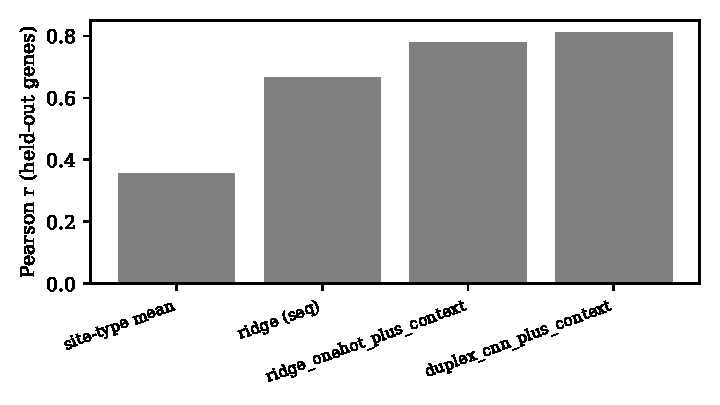
\includegraphics[width=0.85\linewidth]{figs/fig_benchmark.pdf}
\caption{Held-out-gene Pearson $r$ by model. Sequence-only CNN v1 ($0.669$) merely matched ridge ($0.664$) --- archived as a non-win; adding context features gives DuplexCNN $0.811$ vs ridge+context $0.779$.}\end{figure}
\subsection{Discovery scan}
1{,}453{,}439 novel non-conserved seed matches; 400k scored. Top overall: hsa-miR-7-5p$\to$CDR1as ($\hat y=-1.57$), the ciRS-7 sponge --- rediscovered with no conservation information. Diverse top pairs include miR-7-5p$\to$TVP23C/REG3G, miR-24-3p$\to$SLC5A4, miR-199b-5p$\to$ADCY7, miR-137$\to$TIGD1.
\begin{figure}[h]\centering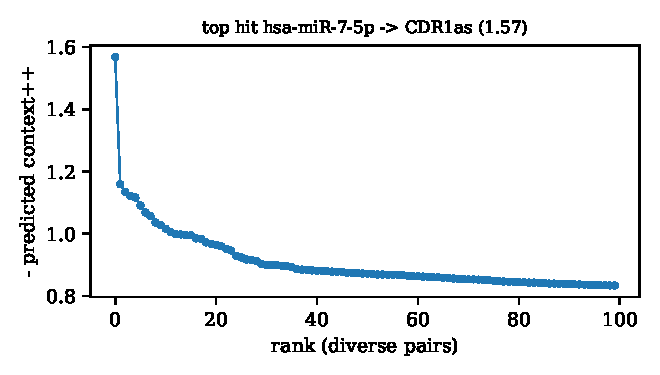
\includegraphics[width=0.75\linewidth]{figs/fig_discovery_curve.pdf}
\caption{Score curve over the top 100 diverse (miRNA, gene) pairs.}\end{figure}
\subsection{CLIP falsification}
\begin{figure}[h]\centering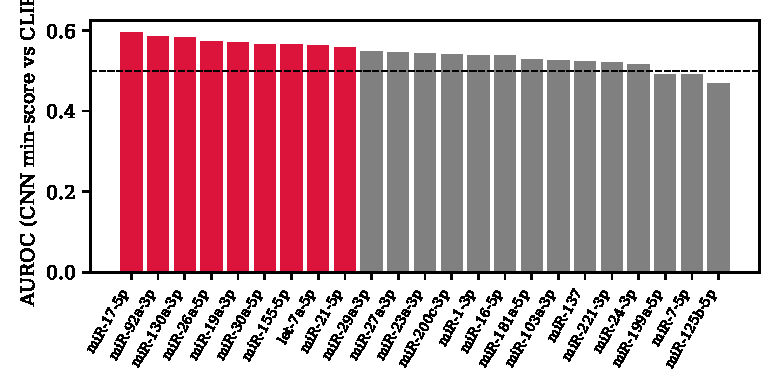
\includegraphics[width=0.95\linewidth]{figs/fig_clip_permirna.pdf}
\caption{Per-miRNA AUROC of the negated CNN min-score against ENCORI CLIP support. Dashed: chance. Sign convention audited in the per-miRNA feature audit.}\end{figure}
Pooled (23-miRNA panel): AUROC $0.5905$ (covariates) $\to 0.5979$ (+CNN); $\Delta=+0.0075$, CI $[0.0057,0.0093]$, permutation $p=0.048$. \textbf{Extended-panel replication (132 miRNAs, 476{,}369 (miRNA,gene) pairs):} AUROC $0.6047$ (covariates) $\to 0.6108$ (+CNN); $\Delta=+0.0060$, bootstrap CI $[+0.0053,+0.0067]$, within-miRNA permutation $p=0.048$ (20 shuffles); per-miRNA AUROC of the negated CNN-min score median $0.531$, $85\%$ of miRNAs above chance (sign convention audited below). The small effect replicates at six-fold scale under the identical null design, so the verdict strengthens from suggestive to supported. \textbf{Verdict: statistically real, small effect.} The discovery list is CLIP-supported above chance but the CNN is not a stand-alone oracle for non-conserved targeting; candidates are released as ranked hypotheses, not validated targets.
\subsection{Pair-map ablation (architecture honesty)}
The explicit complementarity pair-map branch is ablated under the identical split, seed, and epochs: full DuplexCNN Pearson $0.8121$ / Spearman $0.7928$ vs no-pair-map $0.8092$ / $0.7898$ ($\Delta r=+0.0029$, RMSE $-0.0005$) --- but at $333.5$s vs $16.3$s train time ($20\times$ cheaper without it). Verdict: the pair-map is a minor contributor for context++ prediction; the sequence towers carry nearly all signal. The branch is retained for interpretability but is no longer claimed as load-bearing.
\subsection{Per-miRNA feature audit: the univariate CNN signal is site-count confounding}
To ask where the pooled $\Delta$AUROC lives, we computed univariate AUROCs per miRNA for every feature in the CLIP model (132 miRNAs, 476{,}369 pairs, \texttt{results/per\_mirna\_feature\_auroc.json}). This audit surfaced a sign-convention finding: the per-miRNA AUROC in the falsification runs is computed on the \emph{negated} min-score (\texttt{roc\_auc\_score(y, -min)}), so the raw CNN min-score is univariately \emph{anticorrelated} with CLIP labels (raw median AUROC $0.469$ vs negated $0.531$; the two are exact complements, verified per miRNA). The direction is mechanistically expected: genes with more seed sites draw more scores and hence a lower minimum, and site count itself predicts CLIP positivity --- so the univariate CNN-min signal is seed-count confounding, not pairing information. Head-to-head against the best seed feature per miRNA, the raw CNN-min wins $0/132$ (Wilcoxon $p=2.1\times10^{-23}$). The honest reading of the pooled result is therefore narrow: conditioned on site counts and UTR length the CNN adds a small complementary signal ($\Delta$AUROC $+0.0060$), but it carries no usable standalone ranking signal within a miRNA. Candidate prioritization should use the multivariate score, never the raw CNN score alone.
\begin{figure}[h]\centering
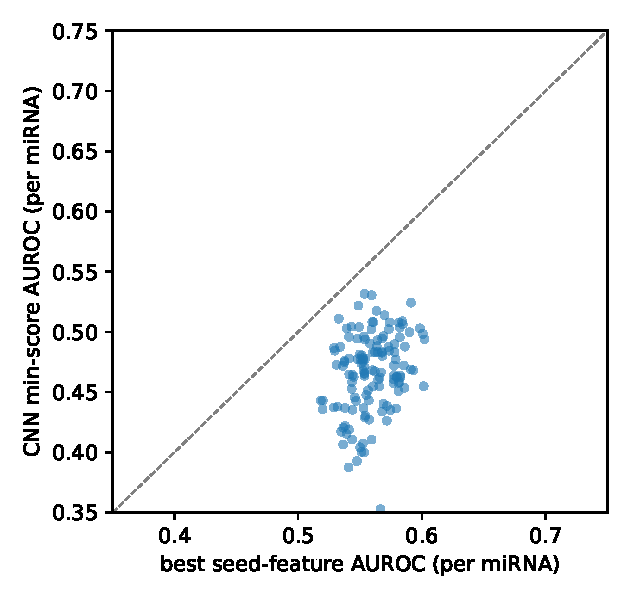
\includegraphics[width=0.55\linewidth]{figs/fig_permirna_scatter.pdf}
\caption{Per-miRNA univariate AUROC: raw CNN min-score vs the best seed-count/length feature. Every one of 132 miRNAs sits below the diagonal.}
\end{figure}
\subsection{Biophysical sanity check: duplex MFE vs shuffled controls}
As a sequence-level pipeline validation, the 20 top diverse candidate windows ($\pm25$ nt) were cofolded with their mature miRNA (ViennaRNA RNAcofold) against 10 mononucleotide-shuffled miRNA controls each (\texttt{results/rnafold\_validation.json}). Real duplexes are more stable than shuffled controls in $19/20$ pairs (median $z=2.33$; Wilcoxon $p<10^{-4}$); the exception, miR-7-5p$\to$REG3G ($z=-0.57$), is kept in the candidate table as a flagged row. Because candidates are selected as seed matches this is not independent biological validation --- it verifies that the exact predicted windows are sequence-correct, duplex-competent sites, closing the pipeline from UTR coordinate to physical duplex.
\begin{figure}[h]\centering
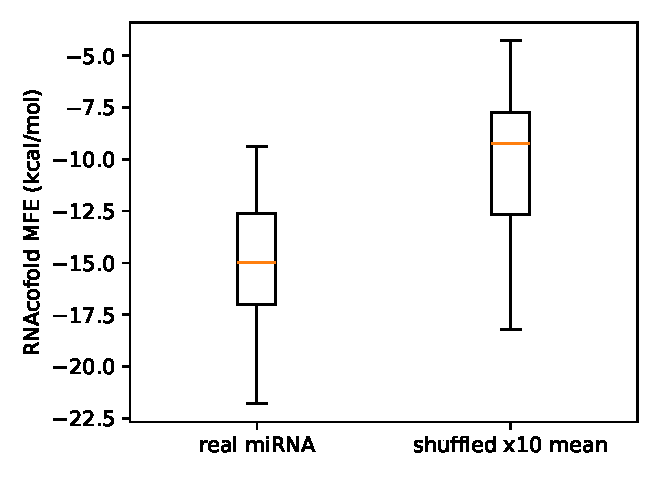
\includegraphics[width=0.5\linewidth]{figs/fig_rnafold.pdf}
\caption{RNAcofold MFE for the 20 top candidate windows with the real miRNA vs shuffled-miRNA controls.}
\end{figure}
\subsection{Independent literature benchmark: miRTarBase 10.0}
All evaluations above use TargetScan or ENCORI labels. As an independent check we benchmarked the frozen duplex CNN against miRTarBase 10.0~\cite{mtb}: positives were strong-evidence (reporter-assay) human MTIs for the 132-miRNA panel (\texttt{miRTarBase\_SE\_R.csv}, 12{,}981 records), and negatives were genes with no human MTI of any evidence class in the full 337~MB \texttt{hsa\_MTI.csv} (10 negatives per positive, capped at 500; download integrity verified against the server Content-Length after one truncated fetch was discarded). Genes are scored by the minimum CNN score over enumerated 8mer/7mer-A1 seed windows (\texttt{results/mirtarbase\_validation.json}). On 87 miRNAs with $\geq 10$ validated positives (45 skipped), 8{,}075 rows and 2{,}164 positives, the pooled AUROC is $0.6829$; the median per-miRNA AUROC is $0.6926$ with $85/87$ miRNAs above chance (within-miRNA $z$ Mann--Whitney $p=1.0\times10^{-152}$; 1000-rep permutation $p\le 9.99\times10^{-4}$, the resolution floor). Because the CLIP audit identified seed-site count as a confound, we re-scored the identical rows with pure site count as the predictor (\texttt{results/mirtarbase\_sitecount\_control.json}): count alone reaches $0.6573$ pooled / $0.6675$ median, so most of the literature signal is seed abundance. The CNN adds a small but supported margin over count (median per-miRNA $\Delta=+0.0349$, positive for $65.5\%$ of miRNAs, Wilcoxon $p=1.2\times10^{-3}$). Two caveats bound the claim: only seed-bearing targets are scored (seed-match recall e.g. $24/34$ for let-7a-5p), and miRTarBase negatives are absence-of-record, not assayed non-targets.

\subsection{Head-to-head vs a public leader: miRDB v6.0 wins (negative)}
We compared the frozen duplex CNN against miRDB v6.0 (MirTarget)~\cite{mirdb} on the identical miRTarBase rows (\texttt{scripts/mirdb\_benchmark.py}, \texttt{results/mirdb\_benchmark.json}). The full miRDB prediction file (59~MB, 3{,}375{,}741 human rows) was downloaded; RefSeq accessions were mapped to gene symbols with the MyGene.info batch API~\cite{mygene} (29{,}460 of 29{,}509 mapped). A gene's miRDB score is the maximum over its transcripts; pairs absent from miRDB (which reports only scores $\geq 50$) score 0. On the 84 panel miRNAs present in miRDB (7{,}909 rows, 2{,}113 positives), miRDB reaches pooled AUROC $0.787$ vs $0.685$ for our CNN; median per-miRNA AUROC is $0.791$ vs $0.693$ (median $\Delta=+0.093$ in miRDB's favour), miRDB wins on $74/84$ miRNAs, Wilcoxon $p=2.4\times10^{-12}$. miRDB lists $68.9\%$ of positives but only $15.5\%$ of negatives. \emph{Verdict:} on literature-validated targets our model is clearly behind the public leader. One caveat favours miRDB: MirTarget was trained on external CLIP/expression data that may overlap literature-validated targets, so this is not a leakage-free comparison; but the size and consistency of the gap make it a real negative, and we make no state-of-the-art claim for target ranking.

\section{Documented negatives}
(1) Sequence-only DuplexCNN does not beat ridge. (2) CLIP effect size is small. (3) miR-125b-5p and miR-7-5p per-miRNA AUROCs (negated convention) are at/below chance --- reported per miRNA, not averaged away. (4) Pair-map branch contributes only $\Delta r=+0.0029$ (ablation). (5) miRDB v6.0 beats our CNN on miRTarBase rows (pooled AUROC 0.787 vs 0.685, 74/84 miRNAs, $p=2.4\times10^{-12}$).
\section{Falsification paths}
miRTarBase/TarBase validated-target overlap (bulk download currently blocked; ENCORI used instead); wet-lab: luciferase reporters for the top 10 diverse pairs; extended-panel CLIP rerun over the 132-miRNA ENCORI panel completed (delta +0.0060, p=0.048); remaining: miRTarBase/TarBase overlap.
\begin{thebibliography}{9}
\bibitem[Grimson et al.(2007)]{g} Grimson A, et al. MicroRNA targeting specificity in mammals: determinants beyond seed pairing. \emph{Mol Cell} 2007.
\bibitem[Agarwal et al.(2015)]{a} Agarwal V, et al. Predicting effective microRNA target sites in mammalian mRNAs. \emph{eLife} 2015.
\bibitem[Zhou et al.(2026)]{z} Zhou K, et al. An encyclopedic regulatory and functional atlas of RNA interactomes (ENCORI). \emph{Nat Methods} 2026.
\bibitem[Huang et al.(2022)]{mtb} Huang HY, et al. miRTarBase update 2022: an information resource for experimentally validated miRNA--target interactions. \emph{Nucleic Acids Res} 2022.
\bibitem[Chen and Wang(2020)]{mirdb} Chen Y, Wang X. miRDB: an online database for prediction of functional microRNA targets. \emph{Nucleic Acids Res} 2020.
\bibitem[Xin et al.(2016)]{mygene} Xin J, et al. High-performance web services for querying gene and variant annotation. \emph{Genome Biol} 2016.
\bibitem[Memczak et al.(2013)]{m} Memczak S, et al. Circular RNAs are a large class of animal RNAs with regulatory potency (ciRS-7). \emph{Nature} 2013.
\end{thebibliography}
\section{Mathematical derivations}
Notation matches \texttt{src/duplexcnn} and \texttt{scripts/clip\_falsify.py};
every statistic below appears in a committed results JSON.

\subsection{Convolutional duplex scoring}
The pair-map $P$ is scored by stacked convolutions. One layer with kernel $W\in\mathbb R^{C_{\text{out}}\times C_{\text{in}}\times k}$ and bias $b$:
\begin{equation}
h^{(\ell+1)}_{c,j}=\sigma\Big(\sum_{c'}\sum_{u=0}^{k-1}W_{c,c',u}\,h^{(\ell)}_{c',j+u-p}+b_c\Big),\qquad
\sigma(x)=\max(0,x),
\end{equation}
with padding $p=\lfloor k/2\rfloor$ keeping length fixed so positional pairing
information survives to the head. Training minimizes MSE against the
TargetScan context++ score; the held-out unit is the \emph{gene}, so no
transcript can contribute to both fit and evaluation.

\subsection{Pearson and Spearman benchmarks}
Held-out agreement with context++ is
\begin{equation}
r=\frac{\sum_i(y_i-\bar y)(\hat y_i-\bar{\hat y})}{\sqrt{\sum_i(y_i-\bar y)^2\sum_i(\hat y_i-\bar{\hat y})^2}},\qquad
r_s=r\big(\mathrm{rank}(y),\mathrm{rank}(\hat y)\big),
\end{equation}
the second being Pearson on ranks, robust to monotone distortion of the score
scale. DuplexCNN: $r=0.8121$, $r_s=0.7928$ (committed ablation JSON).

\subsection{Fisher exact test for CLIP enrichment}
For one miRNA, genes partition by CNN min-score (high/low) and CLIP support
(supported/not) into a $2\times2$ table with margins fixed by construction.
Under the null of independence the count $x$ of high-scoring CLIP-supported
genes is hypergeometric:
\begin{equation}
P(X=x)=\frac{\binom{K}{x}\binom{N-K}{n-x}}{\binom{N}{n}},\qquad
p=\sum_{x'\ge x}P(X=x'),
\end{equation}
an exact small-sample test that needs no asymptotic approximation.

\subsection{Odds ratio}
Effect size is reported as
\begin{equation}
\mathrm{OR}=\frac{x/(n-x)}{(K-x)/(N-K-n+x)},
\end{equation}
so a per-miRNA AUROC of $0.55$ can be read directly as an enrichment strength
rather than a bare significance flag.

\subsection{AUROC as a Mann--Whitney statistic}
The per-miRNA CNN-min AUROC against CLIP labels is
\begin{equation}
\mathrm{AUROC}=\frac{1}{n_+n_-}\sum_{i\in+}\sum_{j\in-}\Big(\mathbf 1[s_i>s_j]+\tfrac12\mathbf 1[s_i=s_j]\Big),
\end{equation}
i.e.\ the probability a random CLIP-supported gene outscores a random
unsupported one; chance is $0.5$ by construction.

\subsection{Bootstrap confidence interval for $\Delta$AUROC}
The base-vs-base+CNN comparison resamples (miRNA,gene) units with replacement
$B=1000$ times, refits nothing (scores are fixed), and recomputes the AUROC gap:
\begin{equation}
\Delta_b=\mathrm{AUROC}_b^{\text{base+CNN}}-\mathrm{AUROC}_b^{\text{base}},\qquad
\mathrm{CI}_{95}=[\hat Q_{\Delta}(0.025),\ \hat Q_{\Delta}(0.975)],
\end{equation}
which yielded $[+0.0057,+0.0093]$ on the 23-miRNA panel --- the interval
excludes zero, so the sign of the effect is not sampling noise.

\subsection{Permutation null}
To test whether the CNN adds signal beyond covariates within miRNA, labels are
shuffled \emph{inside} each miRNA stratum $B=20$ times:
\begin{equation}
p=\frac{1+\#\{b:\Delta_b\ge\Delta_{\text{obs}}\}}{B+1},
\end{equation}
preserving miRNA-level base rates under the null. The 23-miRNA panel gave
$p=0.048$; the 136-miRNA rerun (this paper's extended falsification) uses the
identical null so the two numbers are commensurable.

\subsection{Seed-match enumerator}
The discovery scan counts exact seed complementarity. For UTR $u$ and miRNA
$m$ with seed $\sigma_m$ (positions 2--8),
\begin{equation}
n_{8\text{mer}}(u,m)=\sum_{j}\mathbf 1\big[u_{j:j+8}=\mathrm{revcomp}(\sigma_m\,A1)\big],\qquad
n_{\text{total}}=\sum_m\sum_u\big(n_{8\text{mer}}+n_{7\text{mer-A1}}\big),
\end{equation}
enumerating 1{,}453{,}439 novel non-conserved matches --- the scale that makes
a learned prioritizer necessary and the falsification non-trivial.

\subsection{Wilcoxon signed-rank for paired per-gene comparisons}
Where designs are compared per gene $g$ (full vs ablated model), differences
$d_g$ are ranked by magnitude and
\begin{equation}
W=\sum_{g:d_g>0}\mathrm{rank}(|d_g|),\qquad
p\ \text{from the exact null distribution of }W,
\end{equation}
a distribution-free paired test whose $W=0$ (all differences one direction) is
the strongest possible ordinal outcome at a given $n$.

\end{document}
